
%(BEGIN_QUESTION)
% Copyright 2010, Tony R. Kuphaldt, released under the Creative Commons Attribution License (v 1.0)
% This means you may do almost anything with this work of mine, so long as you give me proper credit

Suppose a thermocouple (producing a DC voltage as it heats up) is connected to a data acquisition module to record the temperature of a process:

$$\includegraphics[width=15.5cm]{i04565x01.eps}$$

The signal recorded by the DAQ unit is ``noisy,'' and you suspect a ground loop in the thermocouple cable.  Explain how you would use basic electronic test equipment (i.e. nothing more complex or specialized than what you would find in our first-year electronics lab) to confirm this was the problem, and also show on the diagram where you would connect this test equipment to perform the confirmation.

\underbar{file i04565}
%(END_QUESTION)





%(BEGIN_ANSWER)

The best answer here is to use an ohmmeter to perform a continuity check (disconnecting the cable shield from the ground terminal and inserting the ohmmeter within that break), because this is the only test that will positively prove or disprove undesired continuity anywhere between the cable's shield and earth ground.

\vskip 10pt

Using an ammeter (connected similarly) is worth half-credit, because while this will show the presence of ground-loop current, the absence of substantial current does not disprove a ground loop.

\vskip 10pt

Using a voltmeter (connected similarly) is worth no credit, because this would show voltage simply due to the cable shield capturing electrostatic interference (as it's supposed to).

%(END_ANSWER)





%(BEGIN_NOTES)

{\bf This question is intended for exams only and not worksheets!}.

%(END_NOTES)

